\documentclass[twocolumn,linenumbers]{aastex631}
\usepackage{amsmath}
\usepackage{booktabs}

% H lines
\newcommand{\halpha}{H$\alpha$}
\newcommand{\hbeta}{H$\beta$}
\newcommand{\hgamma}{H$\gamma$}
\newcommand{\hdelta}{H$\delta$}

%Parameters
\newcommand{\av}{A$_{\text{V}}$}
\newcommand{\mdot}{$\dot{\text{M}}$}
\newcommand{\Mdot}{{\dot{{M}}}}

\newcommand{\msun}{ M_{\sun}}
\newcommand{\rsun}{ R_{\sun}}
\newcommand{\lsun}{ L_{\sun}}
\newcommand{\msunyr}{M_{\sun} \, \rm{ yr^{-1}}}
\newcommand{\kms}{ \, km \, s^{-1}}
\newcommand{\teff}{T$_{\rm eff}$}

% Magnetospheric accretion parameters
\newcommand{\ri}{R$_{\rm i}$}
\newcommand{\rw}{W$_{\rm r}$}
\newcommand{\Dr}{$\Delta \rm r$}
\newcommand{\tmax}{T$_{\rm max}$}
\newcommand{\cosi}{$\cos(i)$}
\newcommand{\lhalpha}{L$_{\rm H\alpha}$}

%\newcommand{\nuria [1]{{\color{green} #1}}}

\received{---- --, ----}
\revised{---- --, ----}
\accepted{---- --, ----}
\submitjournal{}

\begin{document}

\title{Understanding Balmer Decrements in T-Tauri stars in terms of Multi-column Magnetospheric Accretion: Orion OB1b Association}

\correspondingauthor{Naiara Patiño}
\email{nzpatino@bu.edu}

\author[0009-0009-7455-6777]{Naiara Patiño}
\affiliation{Institute for Astrophysical Research, Department of Astronomy, Boston University, 725 Commonwealth Avenue, Boston, MA 02215, USA}

\author[0000-0002-3950-5386]{Nuria Calvet}
\affiliation{Department of Astronomy, University of Michigan, 1085 South University Avenue, Ann Arbor, MI 48109, USA}

\author[0000-0003-1166-5123]{Gladis Magris}
\affiliation{Centro de Investigaciones de Astronomía (CIDA), Mérida, 5101, Venezuela.}

\author[0000-0001-8022-4378]{Marbely Micolta}
\affiliation{Department of Astronomy, University of Michigan, 1085 South University Avenue, Ann Arbor, MI 48109, USA}

\author[0000-0003-4507-1710]{Thanawuth Thanathibodee}
\affiliation{Institute for Astrophysical Research, Department of Astronomy,
Boston University, 725 Commonwealth Avenue, Boston, MA 02215, USA}

\author[0000-0002-5231-7240]{Thomas K. Waters}
\affiliation{Department of Astronomy, University of Michigan, 1085 South University Avenue, Ann Arbor, MI 48109, USA}

\author[0000-0002-5296-6232]{María José Colmenares}
\affiliation{Department of Astronomy, University of Michigan, 1085 South University Avenue, Ann Arbor, MI 48109, USA}


\shorttitle{Understanding Balmer decrements in CTTS using multicolumn accretion}
\shortauthors{Patiño et al.}


\begin{abstract}

    something
    
\end{abstract}

\keywords{stars and stuff}

\section{Introduction}

After the formation of a star from the collapse of a gas cloud, the conservation of angular momentum guarantees the formation of a disk composed of gas and dust around them. These young stars consume material from the circumstellar disk through a procedure known as mass accretion. This is among the most crucial processes that define the evolution of stars and their disks during their initial phases (see \citet{hartmann2016} for a review).

The most well-studied type of young stellar object are the T-Tauri stars which  are low-mass stars of late spectral types \citep{hartmann2016}. Studying the physical processes that occur in these stars, such as mass accretion, is crucial for understanding the evolution of protoplanetary disks and planets. The current paradigm for mass accretion in T-Tauri stars is magnetospheric accretion as described by \citet{hartmann2016}. In this paradigm mass is accreted from the disk in columns following the magnetic field lines of the host star. There is varied evidence supporting this model, such as the UV excess resulting from the shock of the accreted material unto the star \citep{calvet_gullbring1998}  and observed broad emission lines \citep{muzerolle2001}. The study of these emission lines is crucial to the measurement of mass accretion rates of TTS \citep{hartmann1994, muzerolle1998a, muzerolle1998b, muzerolle2001}.


Despite its success, the magnetospheric accretion model has not been able to accurately replicate the observed Balmer decrements, as shown by \citet{micolta2023}. They concluded that this issue seemed like a systematic limitation of the models as they were, likely because of the axisymmetric geometry assumed for the magnetic field. It has been shown that stellar magnetic fields do not follow a simple axisymmetric and dipolar geometry (cite) but an analytical model of a most complex magnetic field is still missing. Given that, in this work we approximate the complex magnetospheric geometry expected in T-Tauri stars with multiple accretion flows of different densities to better explain the observed emission lines. The concept of multicolumn accretion has been applied before to the accretion shock model, and it has been shown to explain NUV and optical emission simultaneously (see \citet{ingleby2013, pittman2022}). There is also evidence of density gradients in the hot spots left on the stellar surface by the accretion columns \citep{espaillat2021} that could indicate an origin in flows of different densities. In this study, we will investigate the concept of multiple accretion columns with varying densities, concentrating on the emissions originating from the flows rather than the shock with the stellar surface.

In this work, we will analyze the observations from  Classical T-Tauri Stars (CTTS) of the Orion OB1b region, previously studied by \citet{manara2021}. This is a appropiate population to study because it is in a intermediate level of disk evolution and it is one of the better studied star-forming region.

This paper is structured as follows. In Section \ref{Sample and observations} we discuss the sample of T-Tauri stars and characteristics of the population, as well as the details and origin of the observational data used. In Section \ref{Models} we expand on the details of the magnetospheric accretion model used to fit the observations. In Section \ref{DataAnalysis} we describe the analysis of the spectral data, corrections, and statistical methods used to obtain our results. Lastly, we discuss those results and their implications in Section \ref{Discussion}.



\section{Observations} \label{Sample and observations}

\subsection{Targets}
The objects studied in this paper are the CTTS of the Orion OB1b association observed in the PENELLOPE Large Program by \citep{manara2021}, as complement to the ULLYSES program \citep{roman-duval2020}. This is one of the closest and most populous OB associations, and their subassociations have ages ranging from $1Myr$ to $10Myr$ \citep{blaauw1994}. The original sample of CTTS consisted of 8 stars with low extinctions ($A_v < 0.3$mag, \citet{briceno2019}). Some of these CTTS were excluded from the final analysis for different reasons. In the case of CVSO 109, it has a reported mass accretion rate of $log(\dot{M})= -6.76\msunyr$, which is outside the accretion model grid used. On the other hand, CVSO 104 and CVSO 165 are binaries and were excluded from the analysis as the individual spectra of their members are not available \citep{manara2021a}. This results in a final sample of 5 CTTS from the OB1b association. For the analysis, we adopted the stellar parameters reported by \citet{manara2021}, which were determined by fitting the object's dereddened spectra with a hydrogen slab model and a photospheric emission template, in order to reproduce the observed excess emission. This method is described in more detail in \citep{manara2013a}. Distances were determined using GAIA EDR3 \citep{gaia2016,gaia2021}. All of these parameters are reported in \ref{ctts_table}. 


\begin{table*}[]
\caption{Stellar parameters of the CTTS sample \citep{manara2021}}

\centering
\begin{tabular}{cccccccccc}

\toprule
Object  & SpT  & $\teff$ [$K$] & L [$\lsun$] & R [$\rsun$] & M [$\msun$] & d [pc] & $\sigma_{err}$ [pc] & Av [mag] & log($\Mdot$ [$\msunyr$])\\ \midrule
CVSO 58 & K7   & 3970                                     & 0.32                         & 1.19                         & 0.81                         & 349.00 & 2.8    & 0.8 & -7.99                   \\
CVSO 90                         & M0.5 & 3700                                     & 0.13                         & 0.88                         & 0.62                         & 338.70 & 3.8    & 0.1 & -7.909                  \\
CVSO 107                        & M0.5 & 3700                                     & 0.32                         & 1.38                         & 0.53                         & 330.40 & 2.5    & 0.3 & -7.32                   \\
CVSO 146                        & K6   & 4020                                     & 0.80                         & 1.84                         & 0.86                         & 332.00 & 1.7    & 0.6 & -8.28                   \\
CVSO 176                        & M3.5 & 3260                                     & 0.34                         & 1.83                         & 0.25                         & 302.40 & 2.9    & 1.0 & -7.38                   \\ \bottomrule
\label{ctts_table}
\end{tabular}
\end{table*}

\subsection{X-Shooter spectra}

The observations were made by the PENELLOPE program with the X-Shooter spectrograph on the Very Large Telescope (VLT) \citep{vernet2011}. This instrument has medium-resolution broad-wavelength coverage and is flux-calibrated. This program was aimed at obtaining complementary data to the ULYSSES program \citep{roman-duval2020}.  Its coverage goes from $\approx 300-2500nm$ permitted to obtain information about the main stellar parameters additionally to the ones describing the accretion process. 

\begin{table*}[]
\caption{Stellar parameters of the WTTS sample}
\centering

\begin{tabular}{ccccccc}
\hline
Nombre          & SpT  & $d$ {[}pc{]} & M {[}$M_*${]} & $T_{eff}$ {[}K{]} & Log $L/L_{\odot}$ & Ref  \\ \hline
TWA9A          & K5   & 68           & 0.81          & 4350              & -0.61             & M13  \\
RXJ1540.7-3756 & K6   & 150          & --            & 4205              & -0.41             & M17a \\
SO879          & K7   & 360          & 1.07          & 4060              & -0.29             & M13  \\
TWA25          & M0   & 54           & 0.84          & 3850              & -0.61             & M13  \\
TWA14          & M0.5 & 96           & 0.73          & 3780              & -0.83             & M13  \\
TWA13B         & M1   & 59           & 0.68          & 3705              & -0.70             & M13  \\
TWA2A          & M2   & 47           & 0.55          & 3560              & -0.48             & M13  \\
TWA9B          & M3   & 68           & 0.37          & 3415              & -1.17             & M13  \\
TWA15A         & M3.5 & 111          & 0.30          & 3340              & -0.95             & M13  \\
Sz94           & M4   & 200          & 0.28          & 3270              & -0.76             & M13  \\
SO797          & M4.5 & 360          & 0.19          & 3200              & -1.26             & M13  \\
Par-Lup3-2     & M5   & 200          & 0.18          & 3125              & -0.75             & M13  \\
SO999          & M5.5 & 360          & 0.13          & 3060              & -1.28             & M13  \\ \hline
\end{tabular}
  % % }
  %   \begin{tablenotes}
  %           \small
  %           % \item \textbf{Nota.} Las distancias reportadas por \citet{Manara2013} y \citet{Manara2017a} se obtuvieron para los objetos de TW Hya por \citet{Weinberger2013, Torres2008, Mamajek2005}, para $\sigma$ Ori de  \citet{Brown1994} y para Lupus III de \citet{Comeron2008}.
  %   \end{tablenotes}

    \label{SP WTTS}
\end{table*}
 
\section{Model} \label{Models}

% Atom2019b:  The lineflux is determined byusing a ray-by-ray method, in which the specific intensity andthe total optical depth of each ray are calculated at a giveninclinationi. Thefinal Hαline profile is calculated from thespatially integrated specific intensity. "

\begin{table*}
\centering
\caption{Model stellar parameters}
\begin{tabular}{ccccc}
\hline
SpT & Teff {[}K{]} & L {[}$L_{\odot}${]} & R {[}$R_{\odot}${]} & M {[}$M_{\odot}${]} \\ \hline
K5  & 4350         & 0.745               & 1.519               & 0.872               \\
K7  & 4060         & 0.515               & 1.451               & 0.726               \\
M1  & 3705         & 0.345               & 1.426               & 0.614               \\
M3  & 3415         & 0.215               & 1.327               & 0.465               \\
M5  & 3125         & 0.117               & 1.171               & 0.306               \\ \hline
\end{tabular}
\label{table:parametros_modelos}
\end{table*}

We use the accretion model proposed by \citet{muzerolle2001} to characterize the emission of the accretion flows and then compare it with the observations. This model  assumes that the magnetic field is axisymmetric and dipolar, with the stellar rotation axis aligned with the magnetic pole. The material from the disk is accreted unto the star in flows or columns chanelled by the magnetic field. The geometry of these columns is defined by a internal radius, which corresponds with the disk's truncation radius, and an external radius, which  in turn determines the width of the flows at their base. This geometry is decribed in  \ref{fig:model_geometry}. This model also assumes a constant mass accretion rate and the temperature at each point is a free parameter and each model is characterized by the maximum temperature.

The expected emission profiles for different magnetospheric parameters were obtained following the method described on the original paper. This uses the extended Sobolev method to simplify calculations and the radiation field is described by a local radiation and a non-local term. From this, it is possible to calculate mean intensities, and then radiative rates used to determine level populations of a 16-level hydrogen atom. Then the specific intensity and optical depth at a given inclination are calculated following a ray-by-ray method. The final emission profiles are obtained by spatially integrating the specific intensity.

Based on this magnetospheric accretion model, we used a model grid of 5 stars with stellar parameters reported in \ref{table:parametros_modelos}. Each of the models of the grid are defined by a combination of magnetospheric accretion parameters: accretion rate ($\dot{M}$), maximum temperature ($T_{max}$), truncation radius ($R_i$), width of the accretion flows at the mid plane ($\Delta R$) and the inclination of the disk ($i$).  The ranges of the parameter space used for this work are described in \ref{table:parameter_space}. We also excluded certain combinations of accretion rates and maximum temperatures from the parameter space following \citet{muzerolle2001}. 

From this grid we calculated the total emission flux of \halpha, \hbeta and \hgamma for each model and then used a six-dimensional linear interpolator to create a way to estimate line fluxes for all combination of parameters inside the defined space. Similarly, we also used six-dimensional linear interpoladors as a way to build profiles of model with any valid parameter combination. It is important to note that the fluxes obtained directly from the interpolators and the fluxes calculated from the interpolated profiles do not coincide for every parameter combination, being the latter the best one to compare to the observations.

\begin{table}[h]
\caption{Parameter space for accretion models}
\begin{tabular}{lccc}
\toprule
Parameter                                              & Min. & Max.  & Step  \\ \midrule
$log(\Mdot$) [$\msunyr$]                           & -10  & -7    & 0.25 \\
$T_{max}$ [$K$]                                           & 6500 & 14000 & 500   \\
$\ri [\rsun] $                                         & 2    & 6     & 0.5   \\
$\Dr [\rsun] $                                     & 0.5  & 2     & 0.5   \\
$i [^\circ]$                                               & 15   & 75    & 15    \\ \bottomrule
\end{tabular}
\label{table:parameter_space}
\end{table}

\begin{figure}
    \centering
    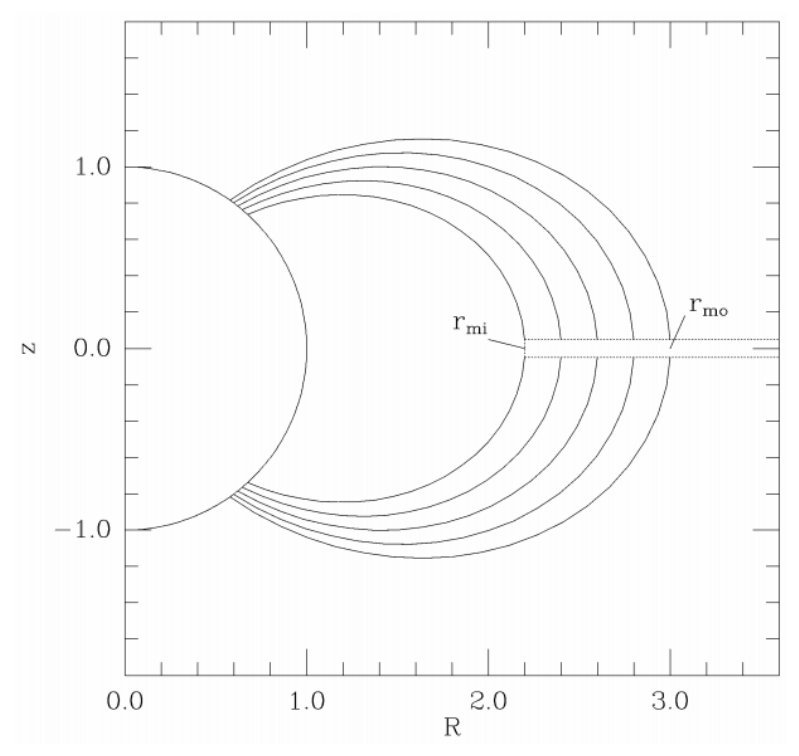
\includegraphics[width=0.75\linewidth]{figures/geometry.png}
    \caption{Model geometry}
    \label{fig:model_geometry}
\end{figure}

\section{Multicolumn accretion}

%atom2019b used two columns in an onion-like structure for a low accretor and could explain observed Halpha profiles

The concept of multiple column accretion has been applied before to the accretion shock model by \citet{pittman2022} and others. They were able to explain observations of shock emission using columns of different energy densities. On the other hand, \citet{atom2019b} used two accretion columns in an onion-like structure to explain observed \halpha profiles of a low accretor.

Several studies indicate that stellar magnetic fields are far from dipolar and axisymmetric (cite). Simulations for more complex magnetic field geometry exist (see \citet{romanova2003}) but an analytical model does not exist (check atom 2023). Using the model grid as is has been insufficient to explain the observed Balmer fluxes in previous works \citep{micolta2023} as it underpredicts \hgamma emission. We try to replicate these fluxes and account more accurately for the complexity of the accretion flows by assuming two accretion columns of different densities. Each would have different emission areas, fractions of the total emission area of the flows. There is supporting evidence of these density gradients in the accretion columns as shown in \citet{zhaohuan2024}.


\begin{figure}
    \centering
    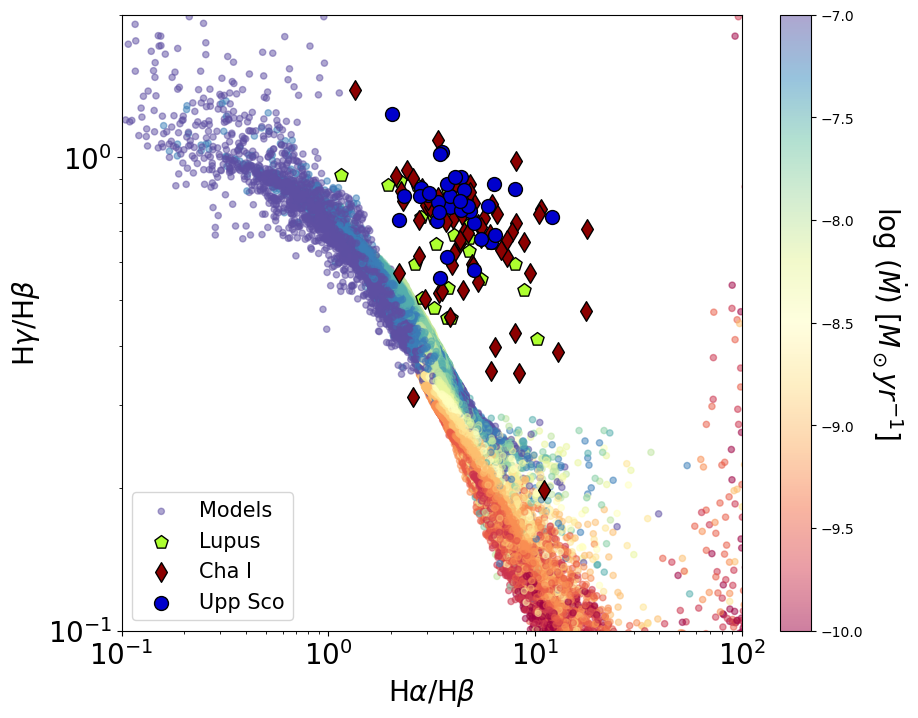
\includegraphics[width=0.8\linewidth]{figures/BalmerDecrements.png}
    \caption{Balmer decrements}
    \label{fig:balmer_decrement}
\end{figure}

The observed Balmer decrements of different regions do not correspond to the Balmer decrements obtained from the model grid, as can be seen in \ref{fig:balmer_decrement}. Given that, we tested whether those could be reproduced by combining the lines fluxes of two different models from the grid weighed by a factor $f_i$ for each model. These factors represent the fraction of the emitting area covered by a given column or accretion flow. We fixed the factor for one of the models $f_1=10^{-3}$ and tried different values of factors for the other model, $f_2 = 10^{-1},10^{-2},10^{-4}$. These factors were chosen based on the \textit{filling factors} of the accretion shock model, which represent the area covered by the shock emission in units of total stellar area. However, it should be noted that the filling factors of the accretion shock model and the $f$ factor of the emitting area of the multicolumn accretion model considered in this work are not equivalent, though they stem from the same idea of the heterogeneity of flows. 

As a test of this idea, we defined a region in the Balmer decrement diagram on which most of the observations fell. Then, we tried different combinations of models and checked if, when weighed by $f_i$, the Balmer decrements of the composited models could reproduce the observed ones, which means that it would fall on the defined region of the Balmer diagram. When looking at the parameter distribution of these two models separately, we can observe certain tendencies. We will refer to each of these models as 'columns' to make the discussion easier. The column covering the smaller area tends to have higher accretion rates, while the larger one tends to have lower accretion rates. That corresponds to a higher density and smaller column and a lower density and larger column.

\section{Data analysis}

\subsection{Observed line fluxes}

Fluxes of emission lines were calculated integrating the spectra after extinction and heliocentric velocity correction and after subtracting the continua determined using this package. The errors were calculated following the method outlined by \citet{alcala2014}. This method consists of determining two more continua, one higher and lower than the middle one. In this case, we used 10\% difference between the central and the other continua. The total line flux was calculated from the average of the flux calculations using the three different continua and the error was the standard deviation $\sigma$. The emission lines analyzed in this work were \halpha, \hbeta and \hgamma.

\subsection{Chromospheric emission}

Due to TTS being magnetically active and having significant UV emission \citep{ingleby2013}, we have to consider chromospheric emission in our analysis. We took this into account by using the spectrum of a Weak TTS (WTTS) of the same spectral type as a template for the chromospheric emission of the accreting stars. The observed spectra of the WTTS were scaled to the CTTS using

\begin{equation}
    F_{WTTS} =  F_{WTTS,obs} \left(\frac{R_{CTTS}}{d_{CTTS}}\right)^2 \left(\frac{d_{WTTS}}{R_{WTTS}}\right)^2
\end{equation}

Where $F_{WTTS}$ is the flux of the WTTS scaled to the CTTS, $F_{WTTS,obs}$ is the observed WTTS spectra, $R_{CTTS}/d_{CTTS}$ the ratio of radius to distance for the CTTS and, $d_{WTTS}/R_{WTTS}$ is the ratio of distance to radius for the WTTS.

\subsection{MCMC}


Although the final goal is to find model combinations that can reproduce the observed emission line profiles, fitting profiles from the entire model grid is computationally expensive and outside the scope of this work. However, we used Bayesian statistics to infer magnetospheric parameters of those model combinations that better reproduce the observed line fluxes to obtain a smaller set of model combinations from which to extract the best fits for the observed profiles. For this first step of flux comparison, our likelihood function is given by:

\begin{equation}
    log (L) \propto -\frac{1}{2} \sum_i \frac{(F_{i,obs}-F_{i,mod})^2}{\sigma_{i}^2}
\end{equation}

where $F_{i,obs}$ is the observed flux of the line $i$, $\sigma_i$ their respective errors, and $F_{i,mod}$ the line flux predicted by the models for that line. The subscript $i$ goes over the three Balmer lines under study: \halpha, \hbeta and \hgamma. The total flux predicted by the models would be the contribution of both of the accretion columns weighted and averaged by the factors $f_i$ added to the estimated chromospheric emission such as

\begin{equation}
    F_{i,mod} = \frac{f_1 \cdot F_{mod,1} + f_2 \cdot F_{mod,2}}{f_1 + f_2} + F_{WTTS}
\end{equation}

We used the \textit{emcee} (cite) package to sample the posterior probability distribution function (PPDF) using the Monte Carlo Markov Chain (MCMC) algorithms. These were run with 50 walkers and 10000 steps to expect convergence of the parameters from which 60\% were discarded as the burn-in steps. Given the complex of the distributions, the option for the \textit{move} algorithm was changed from the stardard of the package \textit{emcee}, from the “stretch move” ensemble method from \citet{goodman-weare2010}, to a more efficient  "DEMove" or Differential evolution proposal, implemented following \citet{Nelson_2014}. 

We use the relationship between $T_{max}$ and \mdot described in \citet{muzerolle2001} as prior, which restricts the parameter space. Finally, for samples with parameters inside the allowed region, the prior is given by a Gaussian centered on the reported \mdot with a width of $1\sigma$. The \mdot 

\subsection{Profile fitting}

We took the final 2200 samples of the MCMC for each star and proceeded to compare the observed profiles to the ones corresponding to each sample. Those were build by adding the contributions of each column weighted by their respective factor $f$ and the scaled flux of the corresponding WTTS for each wavelength. The best fits were found by minimizing $\chi^2$ of the profiles of the three Balmer lines simultaneously. Use inclination to constrict profiles.

After finding the best profiles, we calculated their fluxes to show how they relate to the observed Balmer decrements.

\section{Results}

Previous works using the same model grid, found a systematic underestimation of the flux of \hgamma. One of the goals of this work was to solve this issue using a combination of models. This tries to represent the complexity of real stellar magnetic field by combining high-density and low-density accretion flows covering different fractions of the total area covered on the stellar surface.

Using the MCMC sampler, we were able to find model combinations that could reproduce more accurately observed fluxes of the three Balmer lines studied, solving the issue underestimation of \hgamma.

It appears that \hgamma is forming mainly in the higher density columns, which almost make no contribution to the total flux of \halpha. 

Can we see trends in the parameters of the best fits?

\section{Discussion} \label{Discussion}

Magnetic field geometry is complex, and a one-column accretion model cannot explain the observations. Using two columns we can explain the observed line fluxes. This is a rough approximation to the real complexity of stellar magnetic fields.

Zhaohuan2024: 3D magnetohydrodynamic simulations have shown complex density structure in the accretion flows, such as filaments or an onion-like structure \citep{zhaohuan2024}. Filamentary structures formed by the interchange instability at Rt. These filaments can have densities more than 3 orders of magnitude higher than background density. Multiple accretion columns develop simultaneously and independently from one another. Despite this, mass accretion rate is steady.

Atom2019b: multiple geometrically isolated accretion flows. Two-shell geometry could be reminiscent of a complex structure of the stellar magnetic field. Could be dipolar+multipolar fields (long 2007, 2012). Donati 2007, 2011 dipole and octupole components in V2129 Oph.

Density structure in \citet{zhaohuan2024}, \citet{espaillat2021}

Variability of accretion. "These stars show complicated spectral variability patterns which may be connected with the structure of the magnetospheric flows" \citep{romanova2003}

Magnetospheric flows absorb light from photosphere and chromosphere? \citep{atom2023}

\section*{Acknowledgements}

Thanks Katya

\software{Astropy, ...}

\bibliography{references.bib}{}
\bibliographystyle{aasjournal}

\end{document}
